\documentclass[12pt, twoside]{article}
\usepackage[letterpaper, margin=1in, headsep=0.5in]{geometry}
\usepackage[english]{babel}
\usepackage[utf8]{inputenc}
\usepackage{amsmath}
\usepackage{amsfonts}
\usepackage{amssymb}
\usepackage{tikz}
%\usetikzlibrary{quotes, angles}

\usepackage{graphicx}
\usepackage{enumitem}
\usepackage{multicol}

\usepackage{fancyhdr}
\pagestyle{fancy}
\fancyhf{}
\renewcommand{\headrulewidth}{0pt} % disable the underline of the header

\fancyhead[RE]{\thepage}
\fancyhead[RO]{\thepage \\ Name: \hspace{3cm}}
\fancyhead[L]{BECA / Dr. Huson / 10th Grade Geometry\\* 14 December 2018}

\begin{document}
\subsubsection*{Do Now: Triangle translation}
 \begin{enumerate}

   \item The vertices of $\triangle DAN$ have the coordinates $D(-1,-2)$, $A(2,1)$, and $N(-2,3)$, as shown below. Apply the translation $(x,y) \rightarrow (x+5, y+3)$ to $\triangle DAN$. Draw the image $\triangle D'A'N'$ on the set of axes below, labeling the vertices.
   \begin{multicols}{2}
     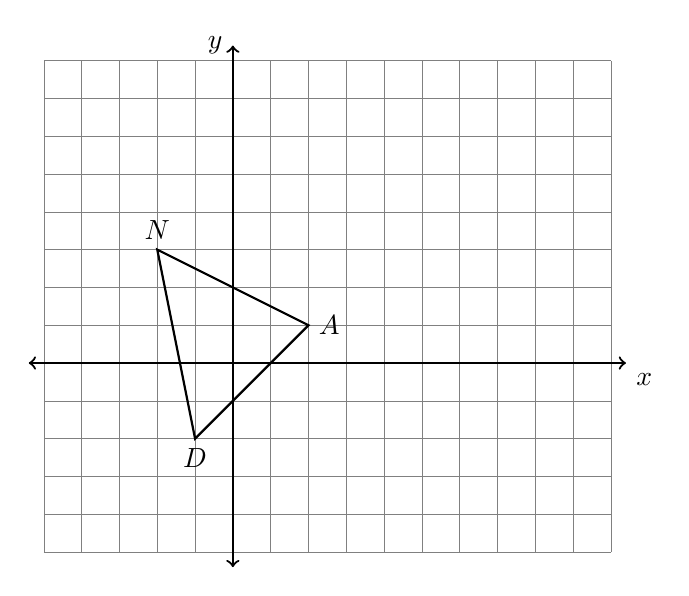
\begin{tikzpicture}[scale=.48]
       \draw [help lines] (-5,-5) grid (10,8);
       \draw [thick, <->] (-5.4,0) -- (10.4,0) node [below right] {$x$};
       \draw [thick, <->] (0,-5.4)--(0,8.4) node [left] {$y$};
       \draw [thick] (-1,-2) node[below] {$D$}--
       (2,1) node[right] {$A$}--
       (-2,3) node[above] {$N$}--
       cycle;
     \end{tikzpicture}\\[0.5cm]
     Which triangle has a larger area, or are they equal in area? Justify your answer.
   \end{multicols}

     \item What is the volume of a rectangular prism (box) with a base measuring 20 centimeters by 12 cm, and 8 cm tall?  \vspace{2.5cm}

    \item What is the volume of an ice cream cone six inches tall and three inches in diameter, \emph{rounded to the nearest whole cubic inch}?  \vspace{3cm}

    \item The air traffic control zone above Kennedy airport is approximately a cylinder with a radius of 1 mile and height of 1,000 feet. What is the volume of the zone, \emph{to the nearest whole cubic foot}?

\newpage
\subsubsection*{Classwork: Circles and angle measures}

\item A round pizza is sliced into five equal slices.
  \begin{center}
  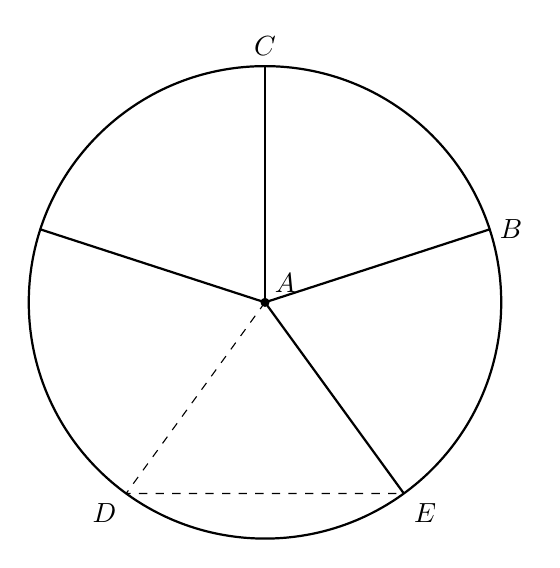
\begin{tikzpicture}
  \draw [thick] (0,0) circle [radius=3cm];
  \draw [fill] (0,0) circle [radius=0.05] node[above right]{$A$};
  \draw [thick] (0,0)--(18:3) node[right]{$B$};
  \draw [thick] (0,0)--(90:3) node[above]{$C$};
  \draw [thick] (0,0)--(162:3);
  \draw [dashed] (0,0)--(234:3) node[below left]{$D$}--(-54:3);
  \draw [thick] (0,0)--(-54:3) node[below right]{$E$};
  \end{tikzpicture}
  \end{center}
  \begin{enumerate}
    \item What is the \emph{central angle} of a slice? (that is, the $m\angle CAB$) \vspace{2cm}
    \item What is the area of the slice? (one-fifth of the pie) \vspace{3cm}
    \item What is the $m\angle ADE$? \vspace{3cm}
  \end{enumerate}

\item Convert $45^\circ$ to radians. (leave your answer in terms of $\pi$) \vspace{1.5cm}

\item Angle $A$ has a measure of 1.2 radians. How much is that in degrees, \emph{rounded to the nearest whole degree}?

\end{enumerate}
\end{document}
